\section{Desarrollo de la Actividad en la M.V.} 
\vspace{\baselineskip}
Al hacer el paso de conectar, se iniciara y podremos visualizar el usuario “Oracle” o también podremos ingresar como root. 
	\begin{center}
		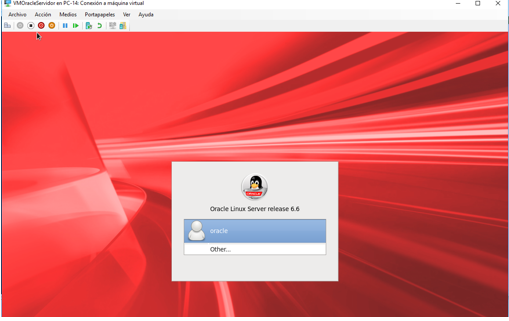
\includegraphics[width=14cm]{./Imagenes/27} 
	\end{center} 

\vspace{\baselineskip}

Nota: \\
Como usuario 2 tenemos al “oracle” y la contraseña es “oracle”. \\
Como usuario 1 tenemos a “root” y la contraseña es “oracle”, todo con minúscula. 
\\
Ingresaremos como usuario 1: root y damos clic en “Login in”.
	\begin{center}
		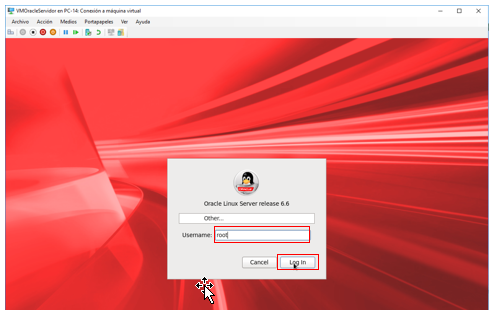
\includegraphics[width=14cm]{./Imagenes/28} 
	\end{center} 

\vspace{\baselineskip}

Ingresamos la contraseña de root “oracle”. Y damos clic en “Login in”.
	\begin{center}
		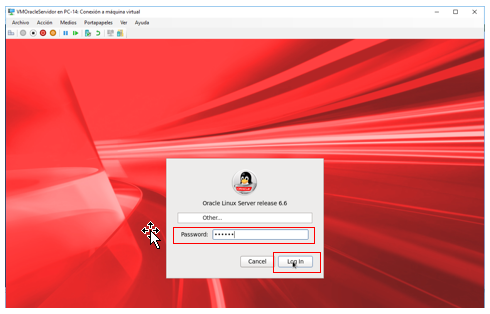
\includegraphics[width=15cm]{./Imagenes/29} 
	\end{center} 

\vspace{\baselineskip}

Ahora pasaremos a colocar una "lps": 
	\begin{center}
		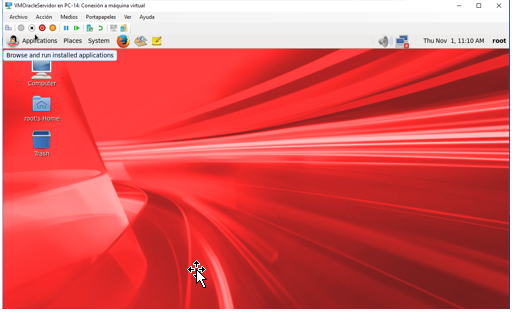
\includegraphics[width=15cm]{./Imagenes/30} 
	\end{center} 

Como vemos asi estará la estructura de la ip:
\begin{itemize}
	\item Ips: 192.168.10.x/24  *  Anfrition: 192.168.10.11  *  Huésped: 192.168.10.12
\end{itemize}

\newpage

En la maquina real vamos a la opción de “Abrir configuración de red e Internet”.
	\begin{center}
		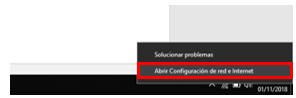
\includegraphics[width=8.6cm]{./Imagenes/31} 
	\end{center} 

\vspace{\baselineskip}

Nos mostrara esta pantalla y escogeremos la opción de “Cambiar opciones del adaptador” 
	\begin{center}
		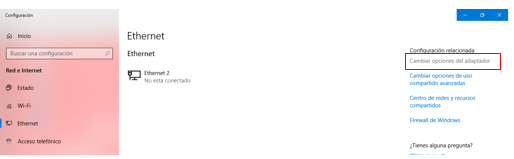
\includegraphics[width=16.5cm, height=6cm]{./Imagenes/32} 
	\end{center} 

\vspace{\baselineskip}

Tenemos que darnos cuenta en el adaptador del Hyper-v y damos clic en “Propiedades”. 
	\begin{center}
		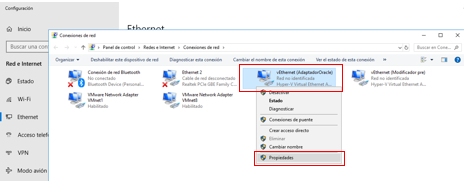
\includegraphics[width=16.5cm,height=6.8cm]{./Imagenes/33} 
	\end{center} 

\newpage

En las propiedades veremos que tendremos que ingresar una ip como muestra la imagen, una vez colocada las ip damos clic en “Aceptar”.  
	\begin{center}
		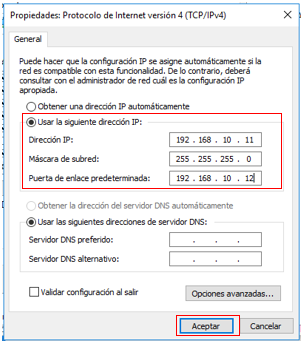
\includegraphics[width=9cm]{./Imagenes/34} 
	\end{center} 

\vspace{\baselineskip}

Ahora pasaremos a la máquina virtual donde buscaremos en la parte superior el siguiente icono y daremos clic en “Edit Connectiones …” damos clic.
	\begin{center}
		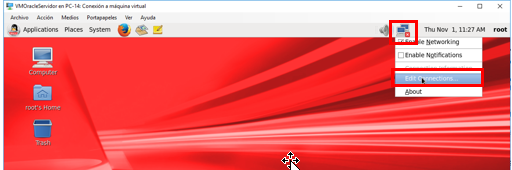
\includegraphics[width=18cm]{./Imagenes/35} 
	\end{center} 

\newpage

Se nos abrirá esta pantalla, primeramente, borraremos el que se encuentra hace años, damos clic en “Delete”.
	\begin{center}
		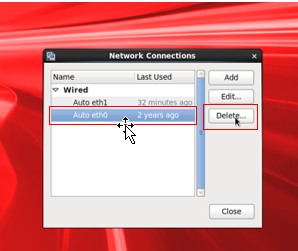
\includegraphics[width=11cm]{./Imagenes/36} 
	\end{center} 

\vspace{\baselineskip}

Ahora editaremos el único que se muestra en pantalla damos clic en “Editar”
	\begin{center}
		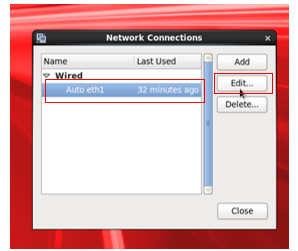
\includegraphics[width=11cm]{./Imagenes/37} 
	\end{center} 

\newpage

Nos mostrara esta ventana en el que ingresaremos la ip que colocamos de la real. Damos clic en “Aply…”.
	\begin{center}
		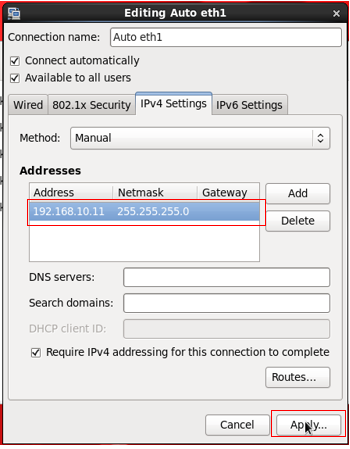
\includegraphics[width=9.5cm]{./Imagenes/38} 
	\end{center} 

\vspace{\baselineskip}

Para poder comprobar que se hizo la conexión de ethernet, abrimos el terminal de Linux, podemos hacer clic derecho en la pantalla y escoger la opción de terminal, cuando ingresemos colocamos el siguiente comando, “ping 192.198.10.11” y damos Enter, en este caso vemos que, si nos está respondiendo de manera correcta, ya que nos retorna una respuesta. 
	\begin{center}
		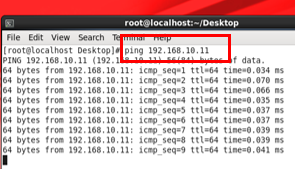
\includegraphics[width=11cm]{./Imagenes/39} 
	\end{center} 

\vspace{\baselineskip}

Como siguiente paso agregaremos el siguiente comando en la que estaremos creando una carpeta. 
	\begin{center}
		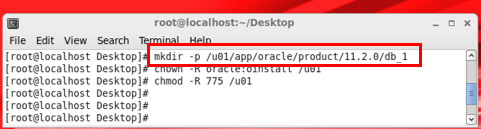
\includegraphics[width=13cm]{./Imagenes/40} 
	\end{center} 

\vspace{\baselineskip}

Luego daremos permiso con el comando “chown” que es usado para cambiar al propietario del fichero. 
	\begin{center}
		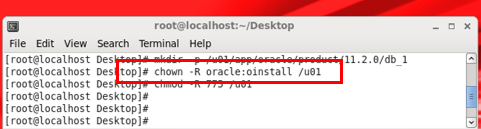
\includegraphics[width=13cm]{./Imagenes/41} 
	\end{center} 

\vspace{\baselineskip}

Daremos permiso otra vez, pero esta vez utilizaremos el comando de “chmod”, este comando permite cambiar los archivos de los permisos de acceso a los ficheros y directorios, se tiene dos métodos para realizar los cambios de permisos: 
\begin{itemize}
	\item Método nivel de control de acceso.
	\item Método octal.
\end{itemize}
Para este caso estamos utilizando el método octogonal. 
	\begin{center}
		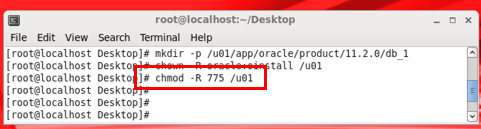
\includegraphics[width=13cm]{./Imagenes/42} 
	\end{center} 

\newpage

Como siguiente paso vamos a configurar algunos parámetros del kernel, para eso será necesario editar el archivo /etc/sysctl.conf ingresando el siguiente comando:
\begin{center}
	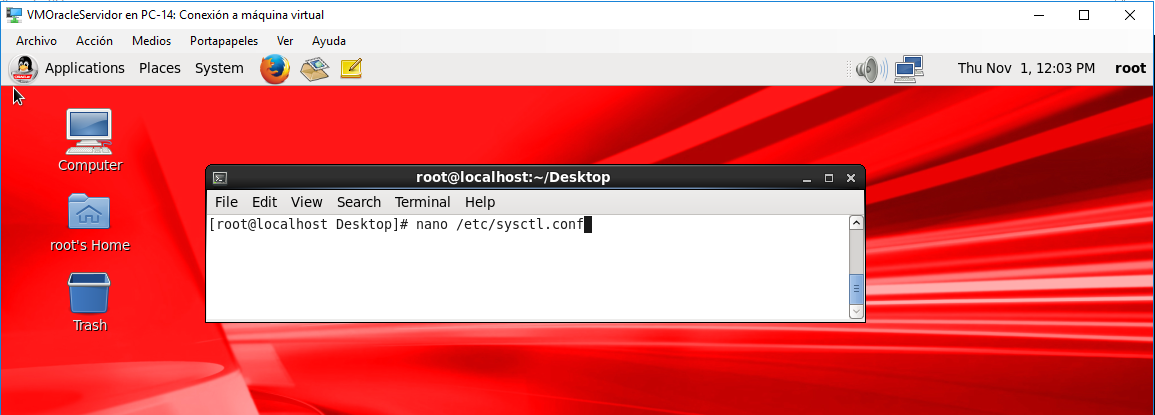
\includegraphics[width=14.35cm]{./Imagenes/43} 
\end{center} 

\vspace{\baselineskip}

Una vez dentro del archivo, añadir al final de este la siguiente información:
\begin{center}
	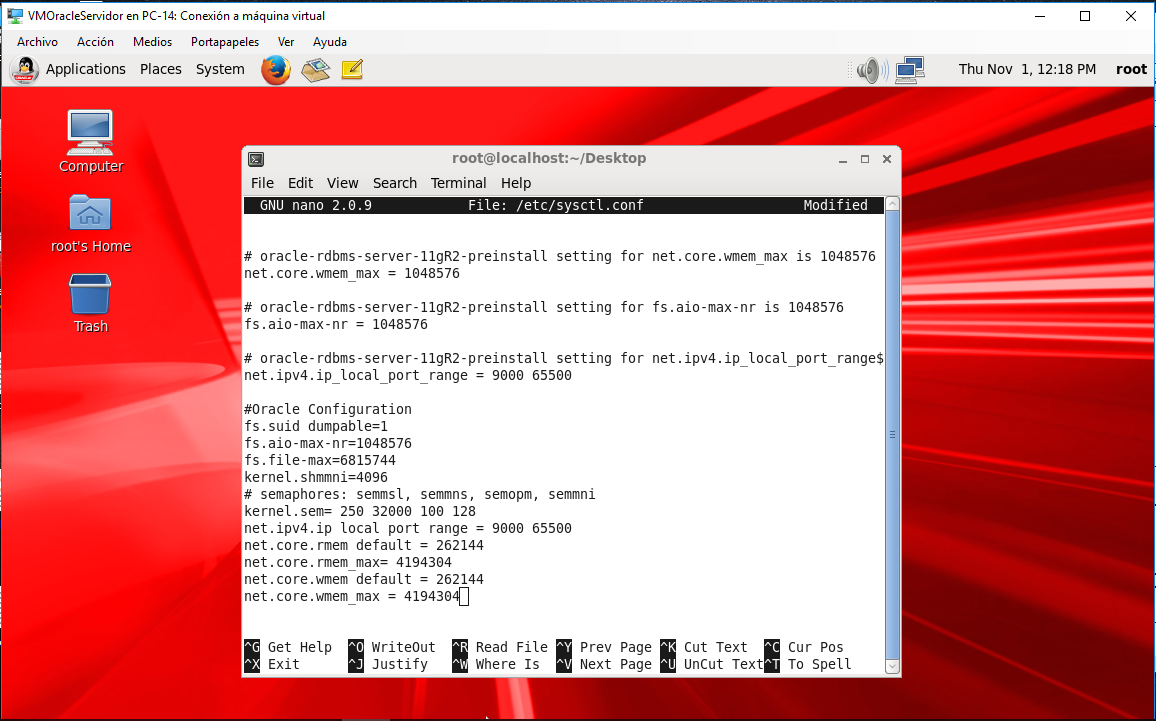
\includegraphics[width=15cm]{./Imagenes/44} 
\end{center} 

\vspace{\baselineskip}

Para salir del editor de textos presionaos la combinación de teclas (CTRL + X) y guardar los cambios. \\
Se deberá ejecutar los cambios realizados, para lo cual ejecute la siguiente sentencia en el terminal.
\begin{center}
	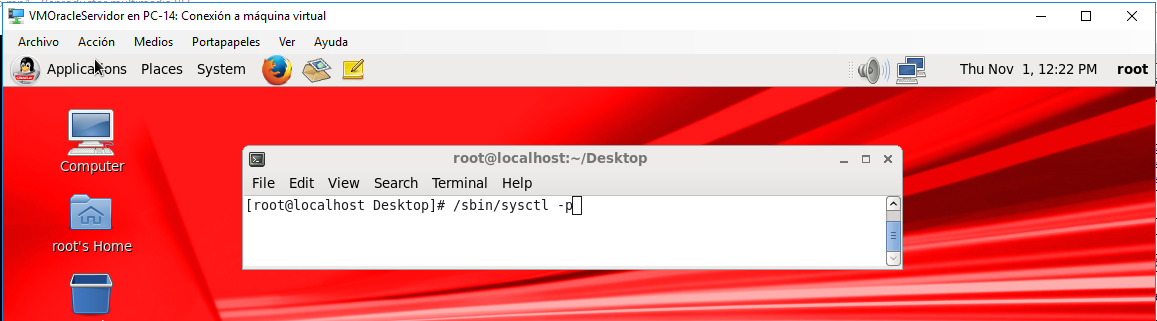
\includegraphics[width=15cm]{./Imagenes/45} 
\end{center} 

\vspace{\baselineskip}

Los resultados deberán ser similares a los siguientes:
\begin{center}
	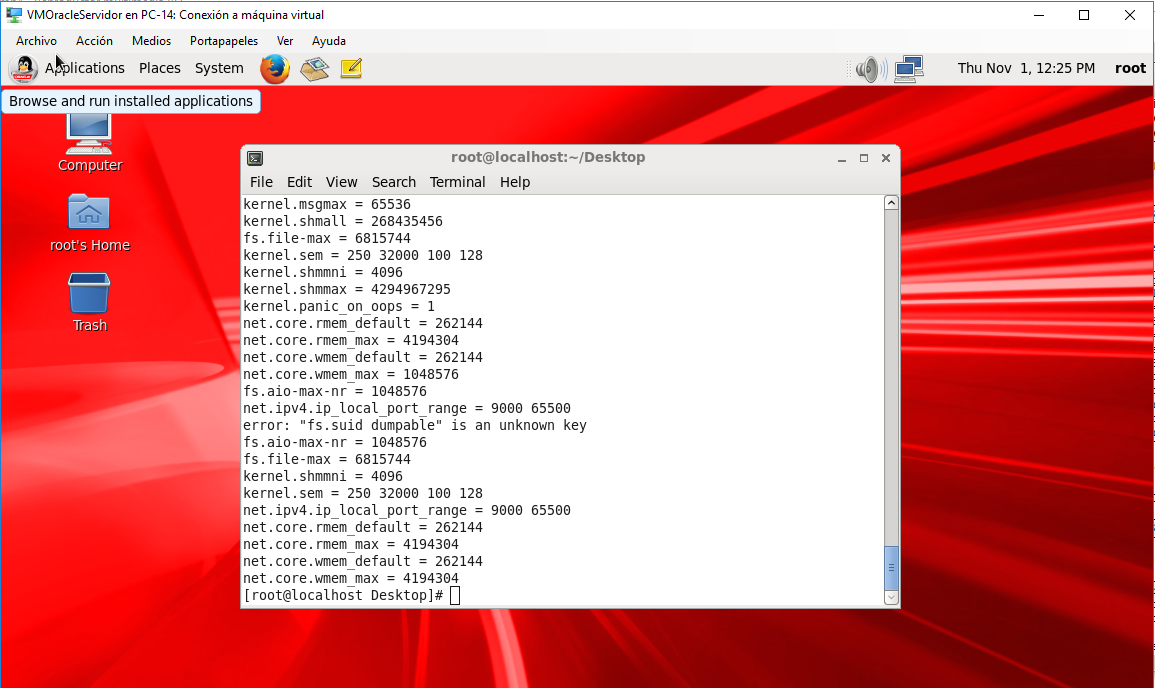
\includegraphics[width=13cm]{./Imagenes/46} 
\end{center} 

\vspace{\baselineskip}

Luego se deberá realizar cambios a los límites de seguridad del sistema para el usuario, para lo cual se debe editar el archivo /etc/security/limits.conf con el siguiente comando:
\begin{center}
	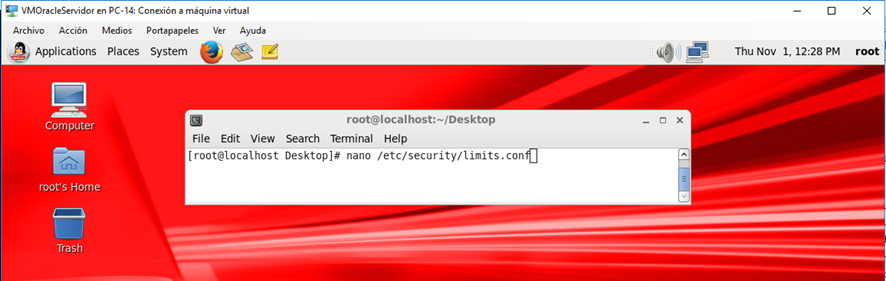
\includegraphics[width=15cm]{./Imagenes/47} 
\end{center} 

\vspace{\baselineskip}

Una vez dentro del archivo, configuramos de la siguiente manera:
\begin{center}
	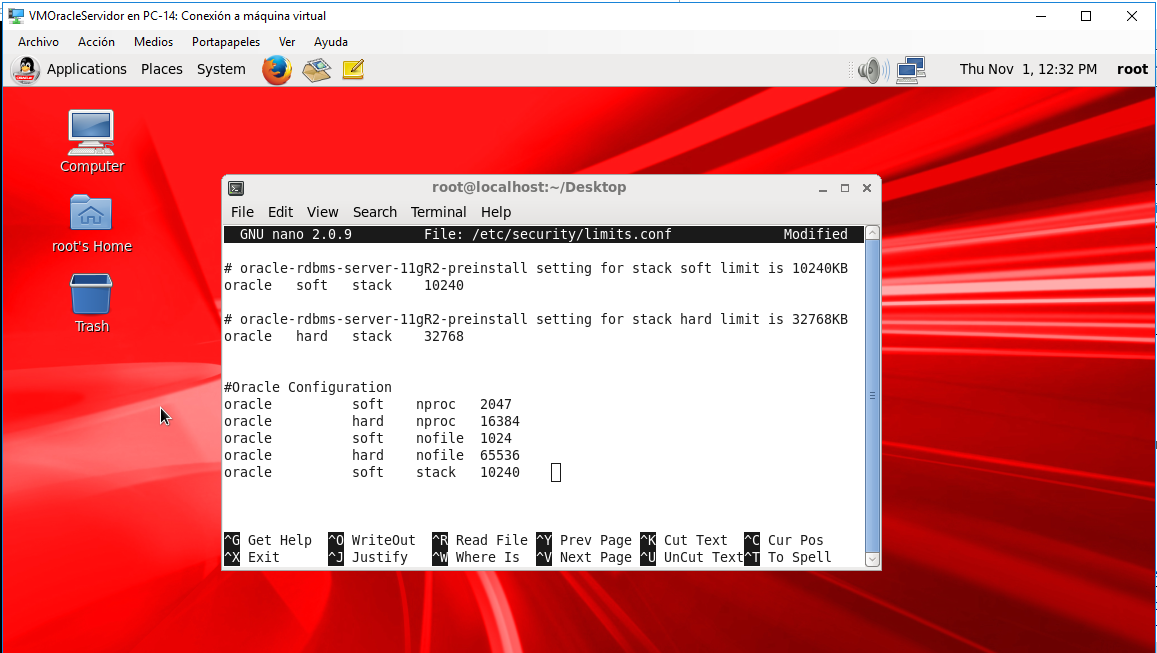
\includegraphics[width=13cm]{./Imagenes/48} 
\end{center} 

\vspace{\baselineskip}

Luego es necesario confirmar que se ha aplicado correctamente la configuración de red, para esto escribimos el siguiente comando: ifconfig eth1
\begin{center}
	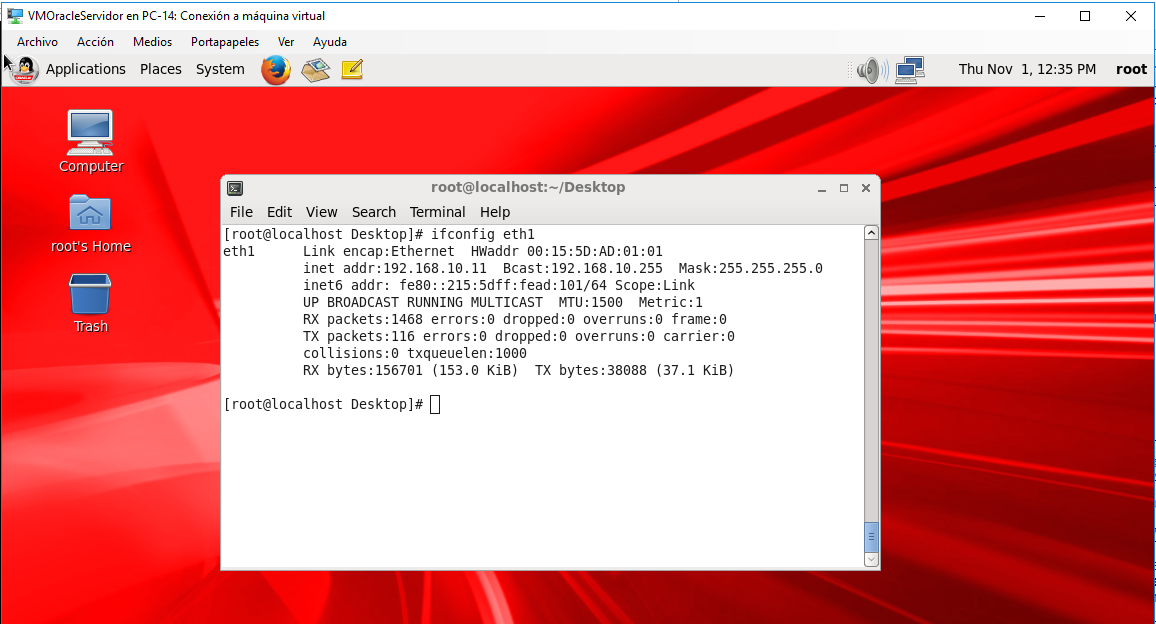
\includegraphics[width=17cm]{./Imagenes/49} 
\end{center} 

\vspace{\baselineskip}

Luego es necesario confirmar que se ha aplicado correctamente la configuración de red, para esto escribimos el siguiente comando: ifconfig eth1
\begin{center}
	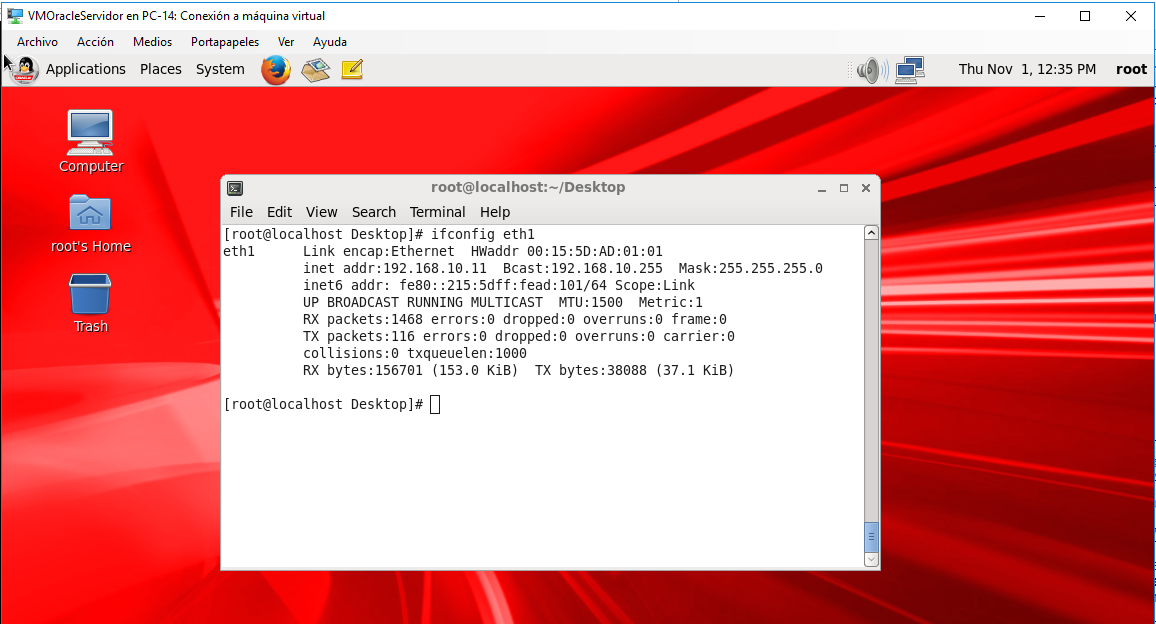
\includegraphics[width=17cm]{./Imagenes/49} 
\end{center} 
El cual debe mostrarnos ese resultado.

\newpage

Luego de establecer satisfactoriamente la dirección IP de la interfaz de red, se debe configurar el nombre del servidor, para lo cual es necesario editar el archivo /etc/hosts (tener en consideración las consideraciones iniciales para establecer el nombre). Se deberá agregar el siguiente comando:
\begin{center}
	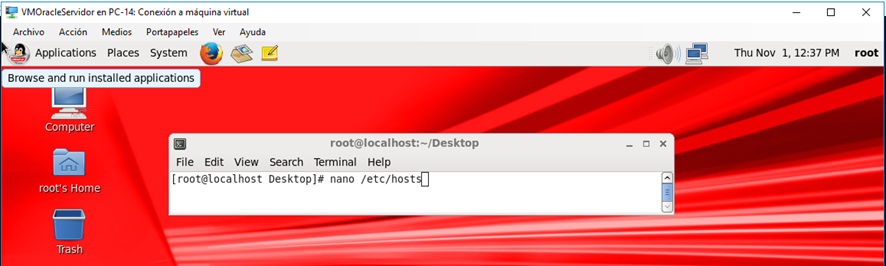
\includegraphics[width=17cm]{./Imagenes/50} 
\end{center} 

\vspace{\baselineskip}

Donde comprobaremos los datos y configuramos de la siguiente manera:
\begin{center}
	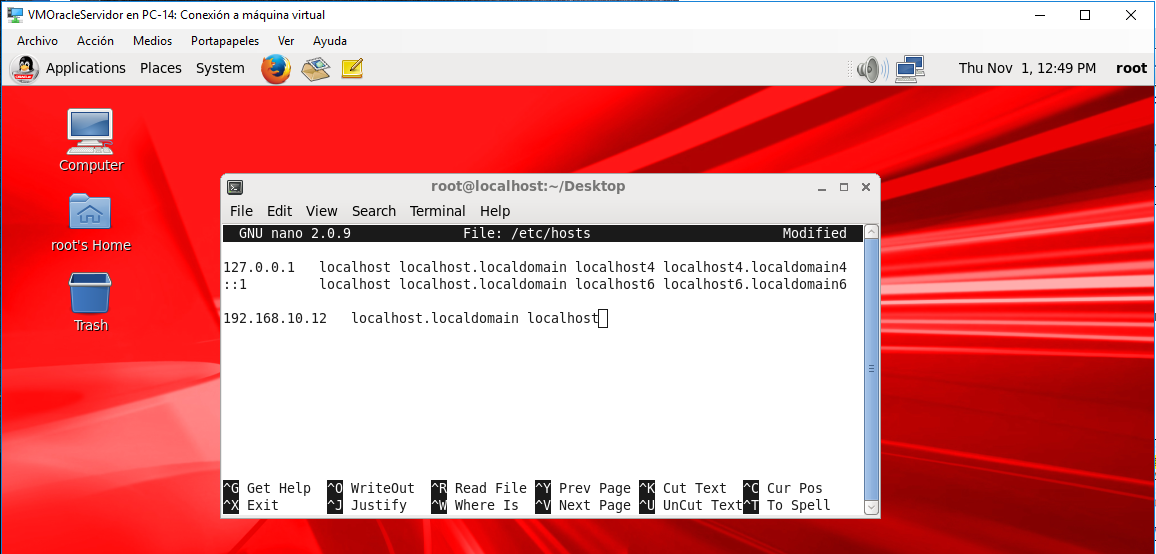
\includegraphics[width=17cm]{./Imagenes/51} 
\end{center} 
Finalmente guardar los cambios en el archivo y cerrarlo.

\vspace{\baselineskip}

Comprobamos que nuestro nombre de host sea el que ingresamos en el archivo de configuración anterior.
\begin{center}
	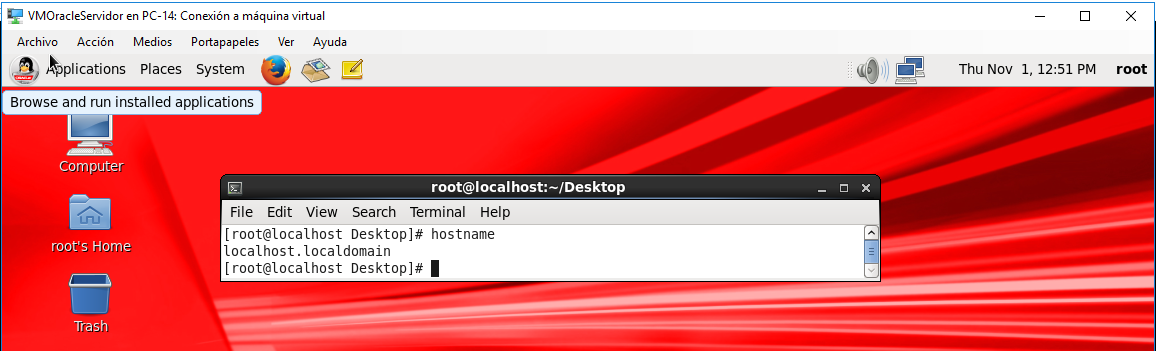
\includegraphics[width=17cm]{./Imagenes/52} 
\end{center} 

\vspace{\baselineskip}

A fin de terminar la configuración del sistema con el usuario “root”, es necesario reiniciar el sistema, para lo cual ingresamos el siguiente comando:
	\begin{center}
		\textbf{\large shutdown -r now}		
	\end{center}
\begin{center}
	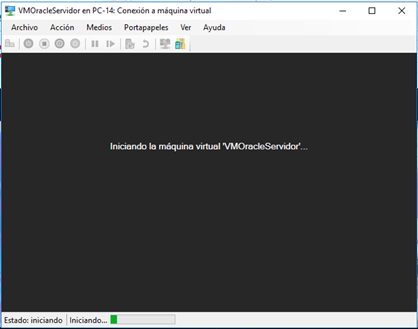
\includegraphics[width=13cm]{./Imagenes/53} 
\end{center} 

\vspace{\baselineskip}

Esperamos a que reinicie el sistema y esta vez nos logueamos como el usuario “oracle”.
\begin{center}
	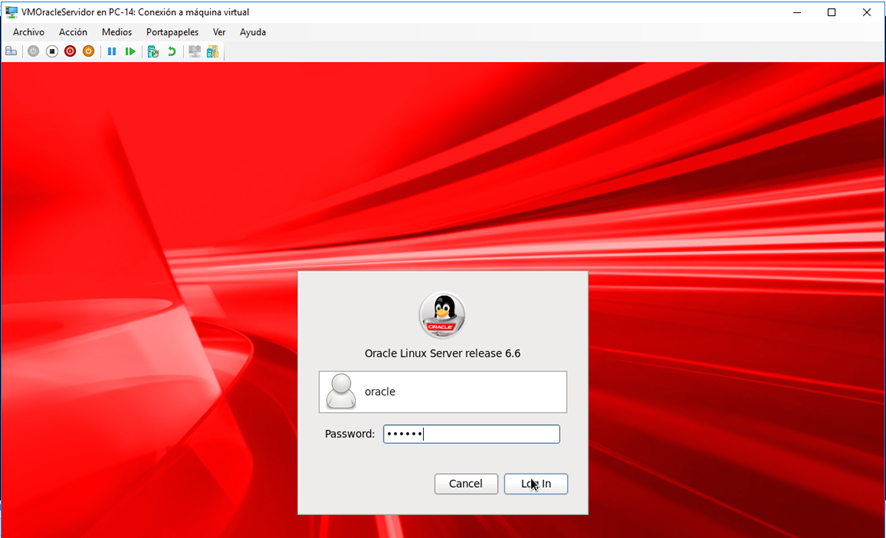
\includegraphics[width=17cm]{./Imagenes/54} 
\end{center} 

\vspace{\baselineskip}

Una vez ingresado con usuario “oracle”, ingresamos al terminal y escribimos el siguiente comando:
	\begin{center}
		\textbf{\large nano .bash profile}		
	\end{center}
\begin{center}
	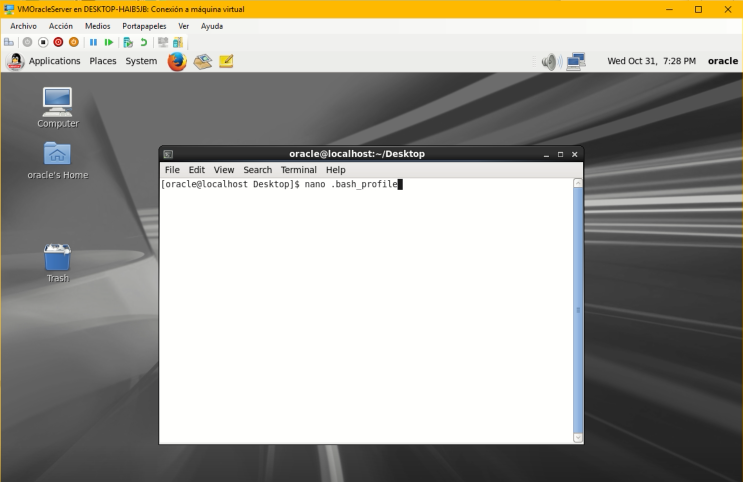
\includegraphics[width=14cm]{./Imagenes/55} 
\end{center} 

\vspace{\baselineskip}

Luego ingresamos el siguiente código de configuración en el archivo abierto.
\begin{center}
	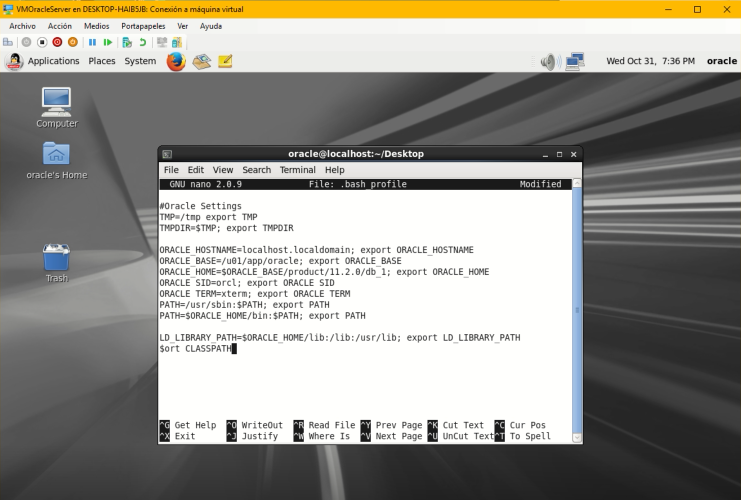
\includegraphics[width=14cm]{./Imagenes/56} 
\end{center} 

\vspace{\baselineskip}

Y volvemos a reiniciar el sistema con el siguiente comando:
\begin{center}
	\textbf{\large shutdown -r now}		
\end{center}



